\chapter{Modernising Rate Monitoring Tools}

This chapter gives an overview of the software development work done to improve and add new features to the CMS Rate Monitoring software. Some other experimental components have ben developed to showcase possible upgrades, delivering quality of life enhancements and enabling shifters and physicists to navigate data in a faster and more comfortable way.

\section{Context}

What are ratemon scripts? How are they used? By whom?

\subsection{ShiftMonitorTool}

The High Level Trigger (HLT) rate monitoring tool is a python script that reports the rates of a selected list of triggers, primary datasets, and streams. The script updates every minute and averages the rates recorded in the last 3 lumisections, and, if possible, compares them to the predicted rate. If a trigger path deviates by a specified amount from the prediction, or exceeds a fixed rate, the corresponding line is highlighted in a yellow colour. The scripts also displays other information that could be useful for the shifter, such as the run number and last lumisections, the LHC status, HLT key, deaditme, instantaneous luminosity and index of the prescale column in use.

\begin{figure}
	\centerline{
		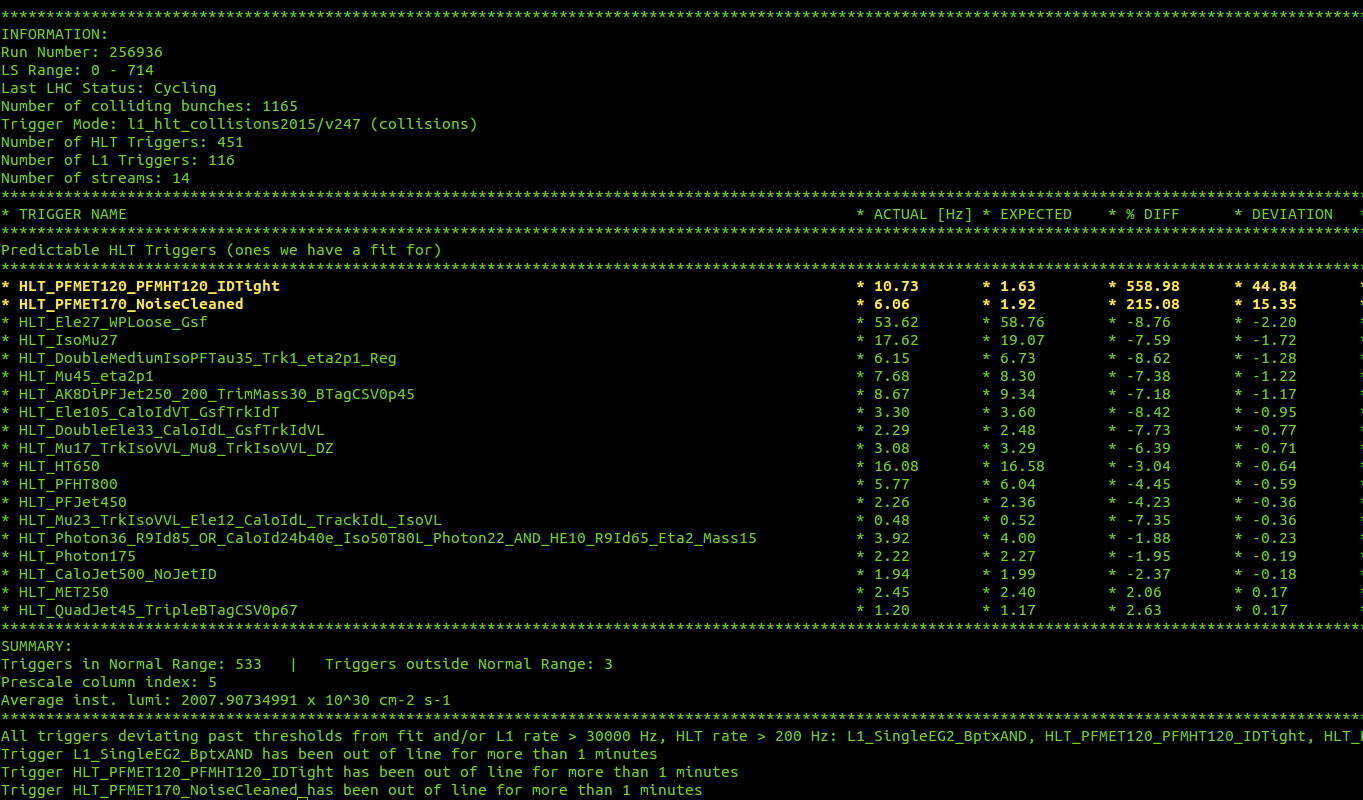
\includegraphics[width=0.8\paperwidth]{figures/ratemon_warnings}}
	\caption{Example execution of the Rate Monitoring Tool showing warnings: two triggers have values consistently deviating from the predictions. \cite{ratemon-twiki}}
	\label{fig:ratemon_warnings}
\end{figure}

\section{Packaging, CI/CD}

To enable CI/CD, we copied the repository on the CERN GitLab. The repository on GitHub is being kept updated but the CI/CD is handled by GitLab.
I've restructured the folder. The "misc" folder now contains the fits logs and the wbmRateReader. The ratemon folder is the only one actually being packaged. The "systemd" folder contains the service file allowing the \texttt{ShiftMonitorTool} to be installed and used as a systemd service.

Docker, GitLab ci, cernbox

Each commit triggers a build and a deployment of a RPM package. This CI/CD system is configured in these files:

\begin{enumerate}
	\item \texttt{.GitLab-ci.yml} - describes the GitLab CI. The first phase (\texttt{build\_rpm}) tells the builder (described by \texttt{builder.dockerfile} and exposed on the GitLab registry) to run \texttt{make rpm} (described in \texttt{Makefile}) and flags the RPM package files as artifacts; In the second phase (deploy), those artifacts are pushed on a EOS folder using the ci-web-deployer tool;
	\item builder.dockerfile - prepares the docker container that will run the build, starting from the cern/cc7-base image. This is exposed using the GitLab registry feature as gitlab-registry.cern.ch/avivace/ratemon/builder;
	\item Makefile - Uses the fpm tool to produce an RPM file with the given metadata and contents. Basically, the ratemon script folder is copied into /opt/ and the systemd service file goes into /usr/lib/systemd/system

	\item The build produces an RPM package file. Those files are pushed during the "deploy" CI phase and finally published on a public CERNBox folder (EOS: /eos/users/a/avivace/ratemon\_builds). This is done using a service CERN account.
\end{enumerate}

Previously, the RateMon tools had to be installed checking out the code from the git repository, running a preparatory script, configuring the database connection and then running the script. Now, the system package manager can install the packaged software.

\section{Configuration}

YAML, schema, database errors?

The ShiftMonitorTool and plotTriggerRates scripts now require an \texttt{--dbConfigFile} option, specifying the YAML configuration file containing the database connection parameters.

I've updated the README and the twiki page to reflect the changes on the DB configuration. Scripts now need to be called in this way:

\texttt{python plotTriggerRates.py --dbConfigFile=dbConfig.yaml --useFills --createFit --bestFit --triggerList=TriggerLists/monitorlist\_COLLISIONS.list 6303}

\section{Exporting data}

JSON, middle db layer?

\section{API}

Connexion, OpenAPI 3 schema, Swagger UI

\section{Web Application}

VueJS, ROOT, Plotly

\section{Integration with OMS}

Highcharts, React, Panel


